\documentclass[prd,preprintnumbers,onecolumn,eqsecnum,floatfix,letter]{revtex4}
\usepackage{color}
\usepackage{calc}
\usepackage{amsmath,amssymb,graphicx}
\usepackage{amssymb,amsmath}
\usepackage{tensor}
\usepackage{bm}
\usepackage{times}
\usepackage[varg]{txfonts}
\usepackage{mathrsfs,amsmath}  
\usepackage{empheq}
\usepackage[colorlinks, pdfborder={0 0 0}]{hyperref}
\definecolor{LinkColor}{rgb}{0.75, 0, 0}
\definecolor{CiteColor}{rgb}{0, 0.5, 0.5}
\definecolor{UrlColor}{rgb}{0, 0, 0.75}
\hypersetup{linkcolor=LinkColor}
\hypersetup{citecolor=CiteColor}
\hypersetup{urlcolor=UrlColor}
\maxdeadcycles=1000
\allowdisplaybreaks
\textwidth 7.5 in 
\hoffset -1 cm 
\newcommand{\boxedeq}[2]{\begin{empheq}[box={\fboxsep=6pt\fbox}]{align}\label{#1}#2\end{empheq}}
\newcommand{\comment}[1]{\textcolor{blue}{\textit{#1}}}
\newcommand{\Sean}[1]{\textcolor{red}{\textit{Sean:#1}}}
\newcommand{\ashok}[1]{\textcolor{cyan}{\textit{Ashok:#1}}}


\begin{document}

\newcommand{\be}{\begin{equation}}
\newcommand{\ee}{\end{equation}}
\newcommand{\ber}{\begin{eqnarray}}
\newcommand{\eer}{\end{eqnarray}}
\def\bea{\begin{eqnarray}}
\def\eea{\end{eqnarray}}
\newcommand{\etal}{\emph{et al.}}


\title{Notes on applying super momentum balance law to constraint GW waveform \\ (Update on Daily Progress) }
\author{Ashok Choudhary}\email{aschoudhary@mix.wvu.edu}
\author{Sean T. McWilliams}\email{sean.mcwilliams@mail.wvu.edu}
\affiliation{Department of Physics and Astronomy, West Virginia University, Morgantown, WV 26506, USA}

\begin{abstract}
\end{abstract}

\maketitle

\section{Local super momentum balance law}

The local super-momentum balance law for asymptotically flat space-time is given by 
\begin{equation}
\mathcal{F}(\theta,\phi) \Big|^{u_{2}}_{u_{1}}  := -\int_{u_{1}}^{u_{2}} du \left[|\dot{\sigma^{o}}|^{2} - \Re\left(\eth^{2}\dot{\bar{\sigma}}^{o} \right) \right](u, \theta, \phi) = \Re\left[\Psi^{o}_{2} + \bar{\sigma}^{o}\dot{\sigma^{o}}\right]\left(u_{1}, \theta, \phi\right) - \Re\left[\Psi^{o}_{2} + \bar{\sigma}^{o}\dot{\sigma^{o}}\right]\left(u_{2}, \theta, \phi\right) 
\end{equation}
where the Weyl scalars is given by,
\begin{align}
	2 \Re\, \Psi^{o}_{2}\left(u, \theta, \phi \right) & = \lim_{r \to +\infty} r^{3} \, C_{abcd}n^{a}l^{b}n^{c}l^{d}\label{psi2}\\  \Psi^{o}_{4}\left(u, \theta, \phi \right) & = \lim_{r \to +\infty} r \, C_{abcd}n^{a}\bar{m}^{b}n^{c} \bar{m}^{d} = \ddot{\bar{\sigma}}^{o} = r\left(\ddot{h}_{+} + i\, \ddot{h}_{\times}  \right)
	\label{psi4}
\end{align}
We simplify the above equation for the case for perturbed black hole using the results in ref \cite{Adamo_2009}. Equation 2.59 in ref\cite{Adamo_2009} is the mass aspect of asymptotically flat space-time. 
\begin{equation}
	\Psi = \psi^{0}_{2} + \eth^{2}\bar{\sigma}^{o} + {\sigma}^{o}\dot{\bar{\sigma}}^{o}
\end{equation}
and the spherical harmonic expansion of the above result is

\begin{equation}
	\Psi = \Psi^{0} + \Psi^{i}Y^{0}_{1\,i} + + \Psi^{i\,j}Y^{0}_{2\,i\,j} + ...
\end{equation} 

Bondi identified the interior mass and three-momentum with the $l=0$ and $l=1$ harmonic contributions is given by
\begin{align}
	M_{B} = \frac{-c^{2}}{2\sqrt{2}\,G}\Psi^{0}\\
	P^{i} = -\frac{c^3}{6\,G}\Psi^i
\end{align}
where $M_{B}$, $P^{i}$ are the interior mass and angular momentum of the space time respectively. Also,
\begin{align}
	Y^{0}_{0} &= 1 \nonumber \\
	Y^{0}_{1\,i} &= -c_i \nonumber \\
	Y^{0}_{2\,i\,j} &= 3c_{i}c_{j} - 2\delta_{i\,j} \nonumber \\
	c_{i} &= -\sqrt{2}\{\cos(\phi)\sin(\theta), \sin(\phi)\sin(\theta), \cos(\theta)\} = -\sqrt{2}\,\hat{r}
\end{align}
Using the above results, equation 1.4-1.7 at leading order we can relate mass and energy momentum of interior space time to $\psi_2$. 
\begin{equation}
	-2\,\sqrt{2}\,M_B -6 \vec{P}.\hat{r} + ... = \Re\left[\psi^{0}_{2} + \eth^{2}\bar{\sigma}^{o} + {\sigma}^{o}\dot{\bar{\sigma}}^{o} \right]
\end{equation}
Here we have just included only the mass and linear momentum terms, further terms includes angular momentum of interior space time (i.e. $J^k = -(\sqrt{2}c^3/12G)\Im(\psi^{0\,k}_{1})$). We can use the above result in the local balance law, to rewrite the local balance law. Substituting $\psi_2$ from equation 1.9 into equation 1.1 and as a first step just considering change in mass we have
\begin{align}
	 -\int_{u_{1}}^{u_{2}} du \left[|\dot{\sigma^{o}}|^{2} - \Re\left(\eth^{2}\dot{\bar{\sigma}}^{o} \right) \right](u, \theta, \phi) =& -\left[\left(2\sqrt{2}M_B + \eth^{2}\bar{\sigma}^{o}\right)(u_1, \theta, \phi) - \left(2\sqrt{2}M_B + \eth^{2}\bar{\sigma}^{o}\right)(u_2, \theta, \phi)\right]\\ = & \int_{-\infty}^{t} du\, \left(2\sqrt{2}\,\dot{M}_B+ \eth^{2}\bar{\sigma}^{o} \right)\\ \implies -|\dot{\sigma^{o}}|^{2} + \Re\left( \eth^{2}\bar{\sigma}^{o}\right) = 2\sqrt{2}\,\dot{M}_B + \eth^{2}\bar{\sigma}^{o} \\ \implies  -|\dot{\sigma^{o}}|^{2}  = 2\sqrt{2}\,\dot{M}_B  
\end{align}
Here we have considered only the mass loss rate to the gravitational wave amplitude. Given the gravitational wave amplitude, above relation can be used to motivate the mass loss rate of interior space time and hence we get a insight for $\psi_2$, which appear in the local super-momentum balance law. 
\section{ Weyl scalar $\Psi^{o}_{2}$ for BOB as perturber cross the light ring }
In Backwards One-Body (BOB) \cite{McWilliams_2019} description of black hole binary merger, the system is described as a single black hole spacetime with a inspiraling in perturber. At the leading order we can just assume that the mass of the perturber and the source is evolving. We first look at how the mass loss rate is related to GW luminosity at leading order for a non-spinning black hole with inspiraling in perturber
\begin{figure}
	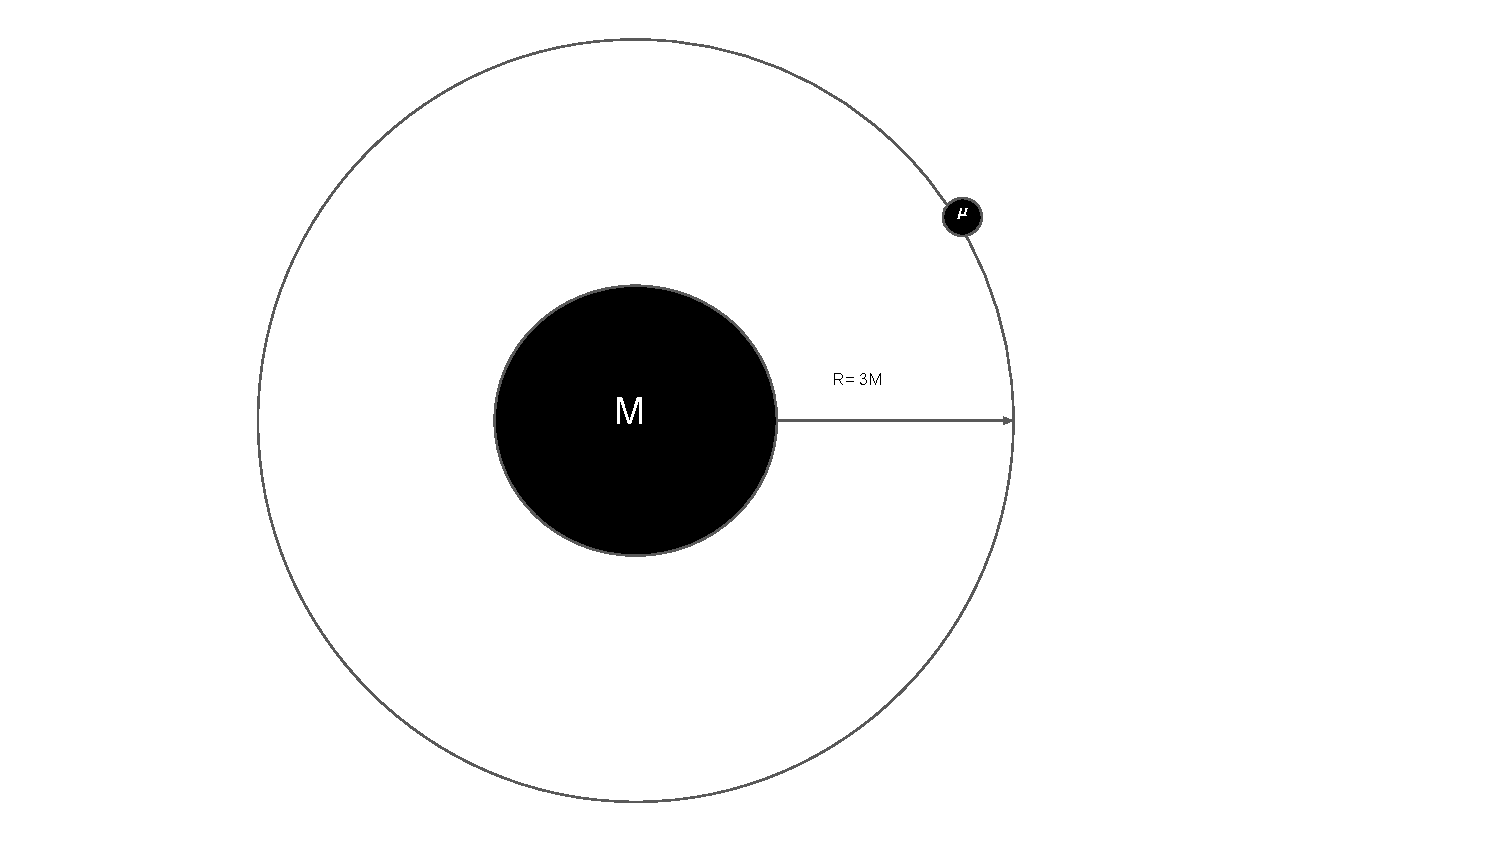
\includegraphics[width=5.5in]{../plots/BOB.pdf}
	\caption{The figure}
	\label{fig:BoBFig}
\end{figure} 
\subsection{Evolution of $\Psi^{o}_{2}$ for perturbed Swarzchild black hole }
We assume that the perturber is loosing mass at given rate $\dot{\epsilon}$. Given this and looking at Bianchi identity on asymptotically flat space time, we can also deduce how the source mass is evolving. One of the Bianchi identity on asymptotically flat space-time is given by 
\begin{equation}
		\dot{\psi}_2 = - \eth^{2}\dot{\bar{\sigma}}^{o} - {\sigma}^{o}\ddot{\bar{\sigma}}^{o}
\end{equation}
The right hand side of the above equation has an asymmetric first term and a symmetric second terms, this motivate us to think of the first terms to be related to inspiraling in perturber and the second terms to be related to the central black hole.\\    
 In this model where we assume both perturber and source mass evolving in time, we want to relate $\epsilon$ to the gravitational strain. We assume the perturber is crossing light right and beyond ISCO the effect of radiation reaction is negligible. In this case the source of gravitational radiation comes from the mass loss by the perturber and the central black hole. Let us look at the expression of luminosity for a inspiraling in perturber at leading order and how it evolves with peturber's mass.
 \begin{align}
 \mathcal{L}_{GW} & = \frac{32}{5}\frac{M^3\,\mu^2}{r^5}\nonumber\\
 \text{let} \;\; \mu \rightarrow \mu - \epsilon \implies \mathcal{L}_{GW} &= \frac{32}{5}\frac{M^3\left(\mu-\epsilon\right)^2}{r^5} \; \; \text{where} \;\; \epsilon \ll \mu\\
 \implies \delta\mathcal{L}_{GW} & = - \frac{32}{5}\frac{M^3\,\mu^2}{r^5}\epsilon\nonumber\\
 \text{Now} \;\; \dot{\epsilon} \propto -|\dot{\sigma^{o}}|^{2} \implies \epsilon &= \int_{t_0}^{t}|\dot{\sigma^{o}}|^{2}dt
 \label{LuminosityMasslossRelation}
 \end{align}         
 
 Now we have the following model for $\psi_{2}$.
 \begin{equation}
 	\psi_{2} = -\epsilon + \frac{d\epsilon}{dt}\int\epsilon\,dt
 	\label{psi2Model}
 \end{equation}


\subsubsection{$\psi_{2}$ \; for different waveform models }

We can use Eqn\;\ref{psi2Model} and \ref{LuminosityMasslossRelation} to construct $\psi_{2}$ for BOB model. Using Eqn. 5 from \cite{McWilliams_2019} we have  
\begin{equation}
	|\psi_4| = A_{p}\text{sech}[\gamma(t-t_p)]
\end{equation}
Since $|\sigma|\approx |\psi|/\omega$ for quasi circular systems. Where $\omega_{l\,m} = m\,\Omega$ and
\begin{equation}
	\Omega = \Biggl\{\Omega^{4}_{0} + k\Big[\tanh\Big(\frac{t-t_p}{\tau}\Big) -\tanh\Big(\frac{t_0-t_p}{\tau}\Big)\Big]\Biggr\}^{1/4}
	\label{Omega}
\end{equation}
where the constant k is given by
\begin{equation}
	k = \Bigg[\frac{\Omega^{4}_{QNM} - \Omega^4_{0}}{1-\tanh[(t_0-t_p)/\tau]}\Bigg]
	\label{k}
\end{equation}

Using Eqn. \ref{Omega} and \ref{k}, at leading order we can relate the mass loss rate to the time derivative of GWs strain. Setting $c = G = 1$ we see that equation 

\begin{equation}
	|\dot{\sigma}|^2 = -2\sqrt{2}\dot{M} = \frac{|\psi_4|^2}{4\Omega^2}
\end{equation}

\begin{figure}
	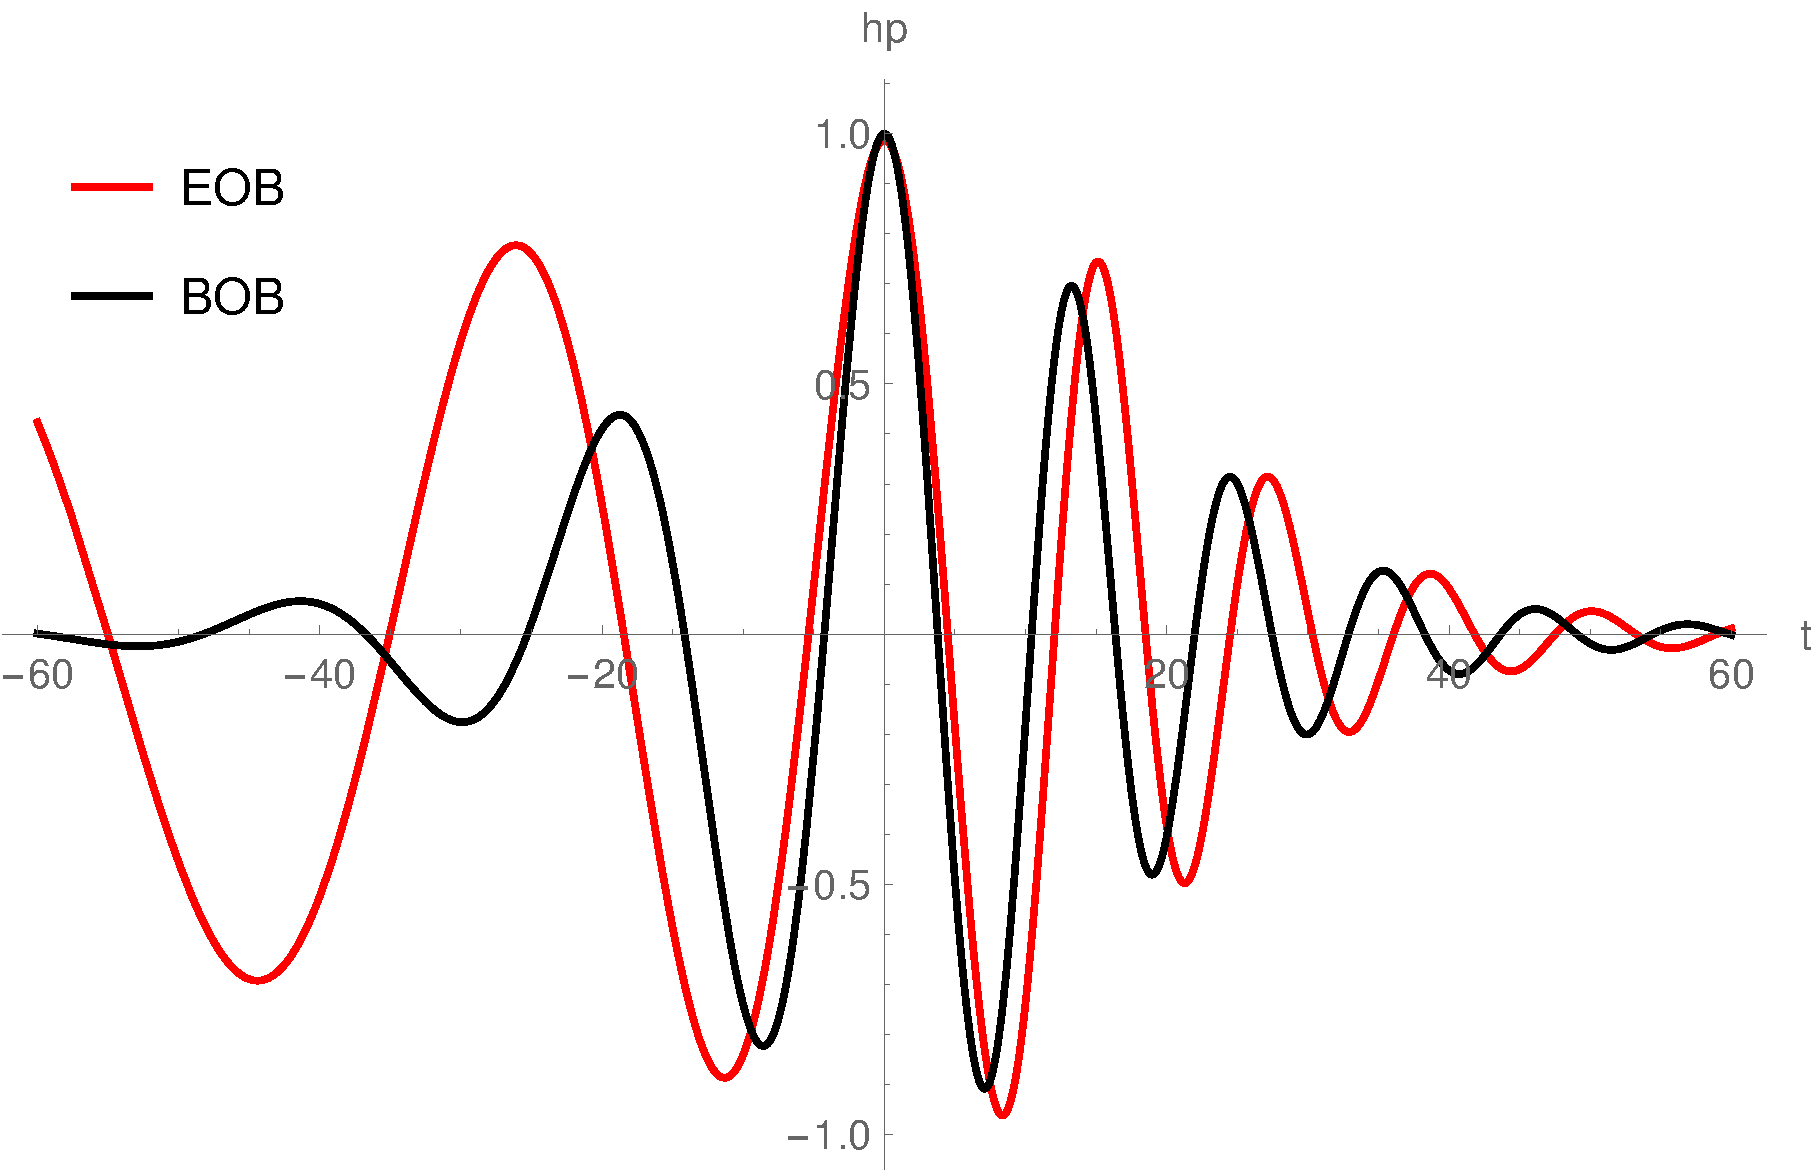
\includegraphics[width=4.0in]{../plots/SigmaSqr.pdf}
	\caption{The figure above shows stain amplitude from BOB}
	\label{fig:SigmaSqr}
\end{figure} 
Using Bianchi identity on asymptotically flat space-time and the expression for $\psi_{4}$
Now for $\sigma$ in the above expression is related to $\psi_4$ in the following way.
\begin{equation}
	\ddot{\bar{\sigma}}^{o} = r\left(\ddot{h}_{+} + i\, \ddot{h}_{\times}  \right)
	\label{psi4} = \psi_{4}^{0}
\end{equation} 
From the BOB model we have the $\psi_{4}^{2\,2}$ 
\begin{equation}
	\psi_{4}^{22} = |\psi_{4}^{22}|\, e^{2i\Phi}
\end{equation}
where $\Phi$ is given by Eqn. 10 in ref\cite{McWilliams_2019}. Now $\psi_{4}^{0}$ is given,
\begin{equation}
	\psi_{4} = \psi^{22}_{4\,\,-2}Y^{22}(\theta, \phi)
\end{equation}
where
\begin{equation}
	_{-2}Y^{2\pm 2}(\theta,\phi) = \frac{1}{8}\sqrt{\frac{5}{\pi}}\left(1 \pm \cos(\theta)\right)^{2}e^{\pm 2\,i\,\Phi}
\end{equation}
Now we can use equation 2.13, 2.15 and the expression for $\psi_{4}$ for BOB in local super momentum balance low. The operator $\eth$ acts on spin-weighted spherical harmonics to increase the spin weight by 1 (i.e $\eth^2 _{-2}Y^{2\pm 2}(\theta,\phi) = \,_{0}Y^{2\pm 2}(\theta,\phi)$, which are the ordinary spherical harmonics). Let us look at each term in local super momentum balance law.
\begin{equation}
	\sigma = h_{+} + i\,h_{\times} = \frac{\psi_{4}}{\omega^2}
\end{equation}   
Since amplitude is slowly varying function of time, each time derivative in the above equation brings one $\omega$ in front. So we have the following relations.
\begin{equation}
	\dot{\sigma}^{0} = \frac{\psi_{4}^{0}}{\omega} 
\end{equation}
So the quantity inside the integral in local balance law can be written as
\begin{equation}
	-\int_{u_{1}}^{u_{2}} du \left[|\dot{\sigma^{o}}|^{2} - \Re\left(\eth^{2}\dot{\bar{\sigma}}^{o} \right) \right](u, \theta, \phi) = -\int_{u_{1}}^{u_{2}} du \left[\bigg|\frac{\psi_{4}^{0}}{\omega}\bigg|^{2} - \Re\left(\eth^{2}\frac{\bar{\psi}_{4}^{0}}{\omega} \right) \right](u, \theta, \phi)
\end{equation}
We can now use $\psi_{4}$ from BOB model. Spin weighted spherical harmonics are independent of time so they can be taken out of integral in the above equation. The above equation can be rewritten as 
\begin{equation}
	-\int_{u_{1}}^{u_{2}} du \left[\bigg|\frac{\psi_{4}^{0}}{\omega}\bigg|^{2} - \Re\left(\eth^{2}\frac{\bar{\psi}_{4}^{0}}{\omega} \right) \right](u, \theta, \phi) = \Re\left(\eth^2 _{-2}Y^{22}(\theta,\phi)\int_{u_{1}}^{u_{2}} du \frac{\bar{\psi}_{4}^{22}}{\omega}(u)\right) - \Bigg|\,_{-2}Y^{22}(\theta,\phi)\Bigg|^2\int_{u_{1}}^{u_{2}} du \bigg|\frac{\psi_{4}^{22}}{\omega}\bigg|^{2}(u)
\end{equation}
The above expression, which is the left hand side of super momentum balance can be written as
\begin{equation}
	P(u_2, u_1, \theta, \phi) =  \Re\left( _{0}Y^{22}(\theta,\phi)\int_{u_{1}}^{u_{2}} du \frac{\bar{\psi}_{4}^{22}}{\omega}(u)\right) - \Bigg|\,_{-2}Y^{22}(\theta,\phi)\Bigg|^2\int_{u_{1}}^{u_{2}} du \bigg|\frac{\psi_{4}^{22}}{\omega}\bigg|^{2}(u)
\end{equation} 
 Let us now look at the right hand side of the super momentum balance law
 \begin{equation}
 	\Re\left[\Psi^{o}_{2} + \bar{\sigma}^{o}\dot{\sigma^{o}}\right]\left(u_{1}, \theta, \phi\right) - \Re\left[\Psi^{o}_{2} + \bar{\sigma}^{o}\dot{\sigma^{o}}\right]\left(u_{2}, \theta, \phi\right) 
 \end{equation}
 We can rewrite the above expression as
 \begin{equation}
 	Q(u_2, u_1, \theta, \phi) = \Re\left[\bigg|\,_{-2}Y^{2 2}(\theta,\phi)\bigg|^{2} \frac{\big|\psi_{4}^{22}\big|^2}{\omega^3}\right]\left(u_{1}\right)- \Re\left[\bigg|\,_{-2}Y^{2 2}(\theta,\phi)\bigg|^{2} \frac{\big|\psi_{4}^{22}\big|^2}{\omega^3}\right]\left(u_{2}\right) 
 \end{equation}
 We can now plot for $P(u_2, u_1, \theta, \phi)$ and $Q(u_2, u_1, \theta, \phi)$ for a given model for $\psi_2$ as a function on initial and final time. For a given waveform the above equation can also be used to show what $\psi$ should look like for a given model. 	
 \begin{equation}
 	\Psi^{o}_{2}\left(u_2, \theta, \phi\right) - \Psi^{o}_{2}\left(u_1, \theta, \phi\right) = P(u_2, u_1, \theta, \phi) - Q(u_2, u_1, \theta, \phi)
 \end{equation}
\begin{figure}
	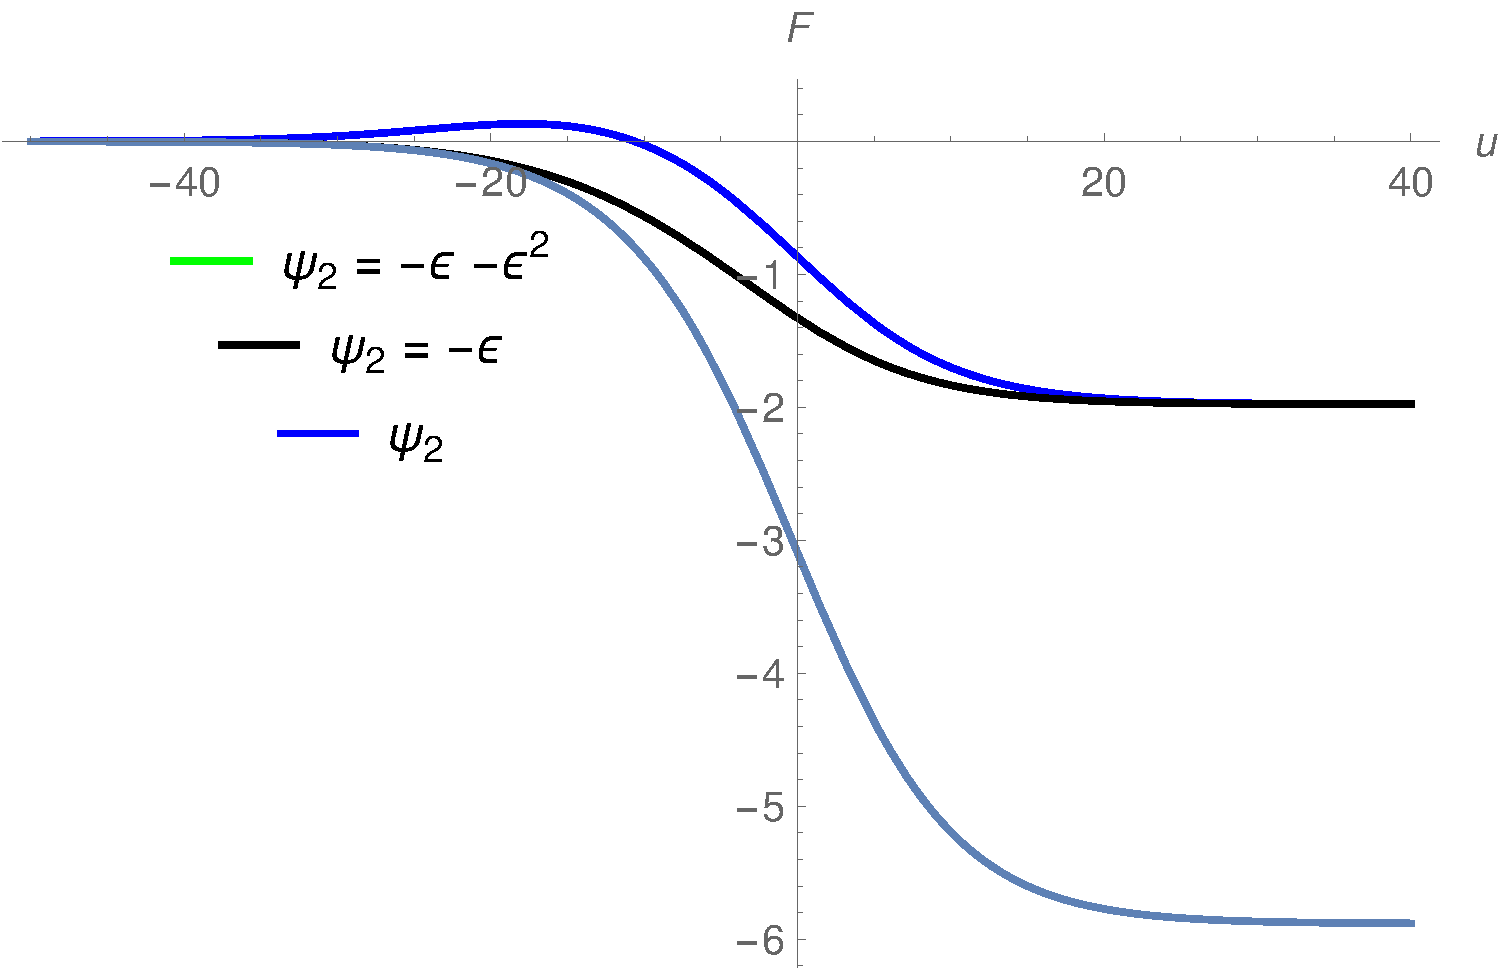
\includegraphics[width=5.5in]{../plots/BalanceLawTwosides.pdf}
	\caption{The figure above show $\psi_2$. The blue curve show $\psi_2$ as it is calculated in Eqn[2.24]. Two other curves shows $\psi_2$ constructed to mass loss in perturber and the black hole.
	$\psi_2 = \int_{t_1}^{t_2}\big|\frac{dh}{dt}\big|^{2}dt$ }
	\label{fig:RHSvsLHS}
\end{figure}
\begin{equation}
	\psi_{2} = -\epsilon + \frac{d\epsilon}{dt}\int_{t1}^{t2}\epsilon \,dt
\end{equation}

\section{Computing $\psi_{2}$ within Effective-One-Body(EOB formalism)}
Computing $\psi_{2}$ with in EOB formalism requires the knowledge of effective metric which includes radiation reaction. This requires mapping between the Post-Newtonian Hamiltonian and the EOB Hamiltonian. Hamiltonian in general are not unique and upto a canonical transformation would give the same equation of motion. The Hamiltonian describing the dynamics of binary using either Post-Newtonian theory or Effective one body should have the same gauge invariant quantities. These gauge invariant quantities includes the binding energy of binary in circular orbit, scattering angle of black holes etc.  In order include the effect of radiation reaction, we begin by looking at the motion of a point particle in some effective metric. The equations of motion can be derived by considering an action in the following way,
\begin{equation}
	S_{point\,mass} -\int d\sigma\left(p_\mu u^\mu - \lambda\left(g^{\mu\nu} p_\mu p_\nu +  m^2\right)\right)
	\label{Action pp}
\end{equation}
where $\sigma$ is some parameter along the worldline of the particle and $\lambda$ is the Lagrange multiplier, which is also a function of parameter $\sigma$. Here the conjugate momentum $p^\mu$ is defined using the particle Lagrangian and the particle velocity in the following way
\begin{align}
	L = &-m\sqrt{g_{\mu\nu}u^{\mu}u^{\nu}} \;\;\text{where} \; u^{\mu} = \frac{dx^\mu}{d\sigma} \nonumber \\
	& \text{and} \; p_{\mu} = \frac{\partial L}{\partial u^{\mu}} \implies L = p_\mu u^\mu
\end{align}
$u_\mu u^\mu \neq -1$ in general since there is not always a one to one mapping between $u^\mu$ and $p_\mu$ for any given parameter $\sigma$. But $p_\mu p^\mu = -m^2$ always holds true and we use this as a constraint in the action defined in eqn [\ref{Action pp}]. 
\subsection{Mapping a two body problem to effective one body}
The usual approach with in Newtonian gravity to map the two body problem to an effective one body requires going into a frame in which there is a central body which has mass equal to the total mass of the system and a smaller body of reduced mass orbiting the central body. In such mapping the total energy and the linear momentum of the system is conserved. In EOB a similar approach is followed, where the motivation to construct an effect one body Hamiltonian comes from fist looking a non interacting two body system and then constructing an effective one body system where preserve the mass shell condition ($p_\mu p^\mu = -m^2$) and conserve the total linear momentum. \\
Consider two non interacting particles with four momentum $p_\mu^1$ and $p_\mu^2$. Now let us construct an effective one body system, which would have a total momentum $P^\mu = p_\mu^1 + p_\mu^2$ and a total mass $M = m_1+m_2$. There is no unique way of defining the relative motion but one valid choice is
\begin{equation}
	p_\mu = \frac{1}{M}\Bigg(\begin{array}{cc}
	-p_{1\mu}p_{2}^\mu \\
	P_0 \overrightarrow{p_1}
	\end{array}\Bigg)
\end{equation}
The definition above has some interesting property that the special part of the momentum reduces to the Newtonian in center of mass coordinates. In COM coordinate frame $P_0$ becomes the $M$ and the time component reduces to the energy of one particle as seen by the frame co moving with the other particle. The above definition gives the following mass shell condition
\begin{align}
	-p_\nu p^\nu &= \mu^2 \;\; \text{where} \; \mu = \frac{m_1 m_2}{M}\\
	-P_\nu P^\nu &= M^2\Bigg[1 + 2\nu \Bigg(\frac{-p_0}{\mu} - 1\Bigg)\Bigg]
\end{align}

The real and effective Hamiltonian are defined as $H = - P_0\nonumber$ and $He = -p_0$ respectively. Using mass shell condition and these definitions for Hamiltonian we have,
\begin{equation}
	H = \sqrt{M^2\Bigg[1 + 2 \nu\Bigg(\frac{H_{eff}}{\mu}-1\Bigg) + \overrightarrow{P}^2\Bigg]}
\end{equation}
   
The relation above is fixed by kinematic mapping between two body system and an effective one body but works quite well even when there is an interaction.  


\section*{References}

\bibliographystyle{apsrev4-1}
\bibliography{references}
\end{document}
